\rule{0.5\textwidth}{0.5pt}\\

	{\large \textbf{EXPERIMENT Euclidean distances for the whole dataset}}\\
	Anova Test p value is 0.0
	\begin{figure*}[ht!]
		\centering
		\subfloat[Euclidean distance cloud]{%
		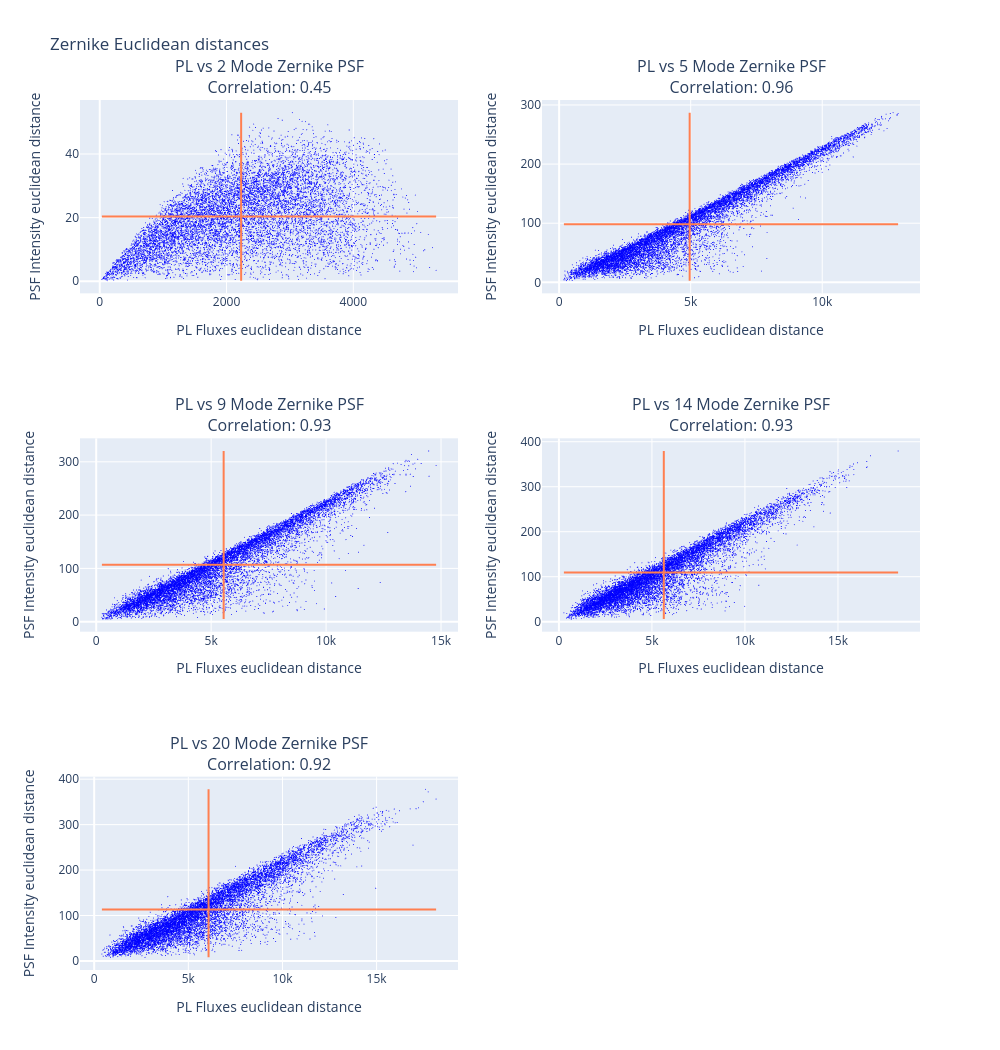
\includegraphics[width=\textwidth]{zernike_euclidean_distances.png}}
		\caption{Euclidean distances ratios between PL and Zernike PSF pairs}\hspace{\fill}
	\end{figure*}
	
	\begin{figure*}[ht!]
		\centering
		\subfloat[Euclidean distance ratios]{%
		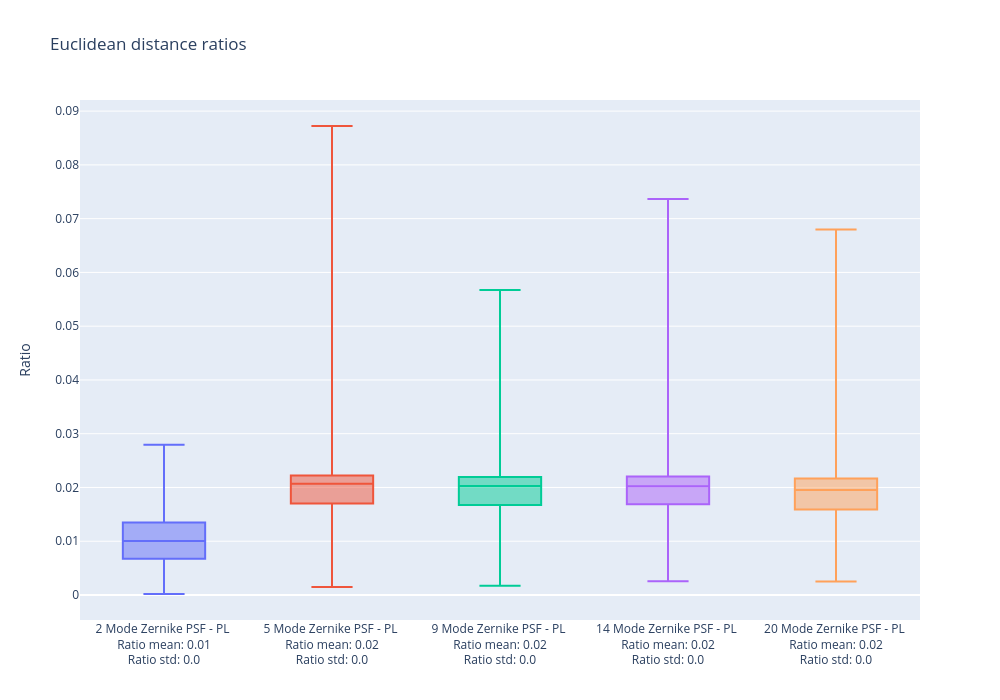
\includegraphics[width=\textwidth]{zernike_euclidean_distances_ratios.png}}
		\caption{Euclidean distances ratios between PL and Zernike PSF pairs}\hspace{\fill}
	\end{figure*}
	
\FloatBarrier	
\rule{0.5\textwidth}{0.5pt}\\